\documentclass{article}
\usepackage[margin=.5in]{geometry}
\usepackage{graphicx}
\usepackage{float}
\usepackage{amsmath}
\newcommand\tab[1][1cm]{\hspace*{#1}}
\usepackage{listings}
\usepackage{hyperref}
\usepackage[utf8]{inputenc}
\usepackage{amsmath} % math libraries
\usepackage{enumitem} %numbering/bullet points
\usepackage[english]{babel}

\begin{document}

\title{Parking Management System Overview}
\author{Ramzey Ghanaim, Jonathan Lam, Mario Cabrera, Travis Rogers} 
\date{Winter and Spring 2018 \\ Parking Management Project} \maketitle

\clearpage
\tableofcontents
\clearpage

\section{Introduction}
\paragraph*{}
The purpose of this project is to design a power efficient parking management 
system that will make parking easier to manage for parking services as well as give users an easier time with finding and paying for parking. The user experience for the project will allow users to feel a sense of pride and accomplishment. See our specs section for a detailed parts list.\\

The project is divided into 3 key pieces as follows:

\subsection{\textbf{Micro Controller and Sensor}} - The micro controller runs off of 3.3V and the sensor runs off 5V so both will require separate power from the same power source using voltage regulators. In order to save power, the micro will control a transistor connecting power to the sensor. This way the micro can be set to a sleep mode periodically which will then stop powering the sensor so that both do not need to be powered constantly. This method will be used while the sensor and micro can be idle and not much activity is going on in the spot. When a car parks in the spot then the next cycle that the sensor and micro are powered then the sensor will send a signal to the micro and the system will stop periodically going into sleep mode so that the micro can supply power to the bluetooth beacon and send data to the gateway using wifi. The string provided by the beacon is used by the app to authenticate the user. When all of the necessary data transfer is done then the micro can continue its cycle of periodically going into sleep mode.\\
The micro controller will also control an RGB LED which will be able to signal to the user if the spot is empty, taken, or illegal. Initially parking and blocking will trigger the proximity sensor. This will start a timer, and after a certain amount of time then the sensor can assume that a car is parked. This way the sensor does not think that a car is parking and leaving every time that someone walks in front of the sensor and also helps debounce to eliminate noise. After a certain time, if there has been no bluetooth connection and the spot is still blocked then the unit can assume that there is an illegally parked car in the spot and can signal the gateway and cloud to alert parking services. 

\subsection{\textbf{Mobile Application}} - The mobile application we will develop allows the user to claim his/her spot and validate the necessary permit or charges. When the user first opens the app while in a parking spot, the phone's blue tooth sensor will receive the blue tooth string given off by the micro controller. The string and user account information will be sent to the cloud from the app. The app will then wait for verification from the cloud. Once the information has been received back from the cloud a display will open for permit/payment information. A similar process then happens again, this time confirming whether or not the parking is legal.
\\
The app layout will rely an a simple navigation drawer with an action button. The navigation drawer will list out the number of different parking lots the user can choose from, and the action button will be used to receive and send the proper bluetooth beacon. The navigation drawer is composed of pages known as fragments. Each map fragment will show a birds eye view of the designated parking structure with each parking space shown as either ``open" (colored green) or ``taken" (colored red). The app will allow the user to zoom in and out of the map and see which spaces are available any time, from anywhere. The action button is intended only when the user has found a parking spot. If the button is accidentally pressed when the user is not in his or her preferred parking spot, the bluetooth verification may not go through. If it does go through however, the user has the option to cancel the specified parking spot in the payment menu.

\subsection{\textbf{Database and Cloud Computation}} - The cloud will receive data from the micro controller gateway and the app to verify a spot is being blocked, the user is in the spot being blocked and the user has a valid parking permit associated with his/her account. The cloud is based on the Google Cloud Platform which has excellent integration with a SQL database of users, parking spots, and history.

\section{Specifications}
\subsection{Sensor}
The sensor we are using is the HC-SR04 Ultrasonic Module. The module uses 4 5V pins. The pins are as follows:
\begin{enumerate}
\item \textbf{VCC} - Power is supplied through the VCC pin.
\item \textbf{GND} - The sensor is connected to ground through the GND pin.
\item \textbf{TRIG} - The sensor sends out an ultrasonic wave when we send a $10 \mu s$ length pulse to the trigger (TRIG) pin.
\item \textbf{ECHO} - When a wave is reflected back, a pulse is sent to the ECHO pin. \\\\
\end{enumerate}
\subsection*{} When in an active state, the micro controller will both send a $10 \mu s$ pulse through the sensor TRIG pin and start a counter. When the pulse is reflected back to the sensor, it will send a signal back to the micro controller through the ECHO pin. The echo pin will trigger an interrupt in the micro controller. During this interrupt, the counter will be stopped and we will use the time and the speed of sound to calculate the distance of an object. Our goal is to detect objects within 3 feet of our sensor. \\
Since the micro and the sensor require different voltages to run properly, we have decided to use op amps to allow the voltages to travel across the sensor and micro without one harming the other device. For the TRIG pin, the micro will send the 3.3V pulse through to an op amp with a gain of 1.52 so that the output voltage will remain 0 when no pulse is sent and amplify from 3.3 to 5V for the pulse. The ECHO pulse will need to have a gain less than one which can be done with either an op amp or a simple voltage divider. Either way we will need to drop the ECHO pulse voltage by a factor of .66 so that the voltage coming into the micro does not go far above 3.3V and possibly damage a pin.

\subsection{Cloud Computation}
To facilitate communication between the sensor gateways, database, and user application, we use Google's App Engine to compute the application logic and provide connectivity between devices. The platform allows us to respond to sensor updates and trigger verification events when cars enter the parking spot. It also executes the steps needed to verify the user's parking spot using the app and services payments. Each interaction between the App Engine and the other devices are listed below:
%\begin{enumerate}
\subsubsection{\textbf{Gateway}} - The gateway aggregates all the sensor information from the micro controllers and sends the data to the App Engine. The gateway will wrap the data in a HTTP POST message in the form of a text string. The App Engine will receive the POST message and extract the sensor data, triggering a verification event for recently blocked sensors and saving sensor states to the database.
\subsubsection{\textbf{Database}} - The App Engine will receive and send any needed data from the database using SQL commands, such as updating the state of the parking space or writing event logs into the database.
\subsubsection{\textbf{User App}} - The user app connects to the App Engine URL with the Bluetooth Beacon data using HTTP POST message. The App Engine matches the Bluetooth Beacon's unique string with the blocked spot to verify the user's occupation of the parking spot. It then responds by either confirming the status of the sensor to taken or responding with payment options.
%\end{enumerate}
%%%%%%%%%%%%%%%%%%%%%%%%%%%%%%%%%%%%%%%%%%%%%%%%
\subsection*{} When a micro controller determines that a spot is occupied, the sensor status is changed and sent to the gateway. The gateway will aggregate the data from its connected micro controllers and send them to the Cloud App Engine as an HTTP POST, triggering a verification event. The mobile App will read the Bluetooth Beacon string from the micro controller and send the data to the App Engine, which will matches the Bluetooth string from the user with the blocked spot's unique string. If valid, the App Engine will access the database and check if the user has a parking permit. The App Engine will send a success message back to the user app indicating a successful parking if valid, or indicate a payment option for those without a permit. If the user does not complete a payment option by a certain period of time, such as 10 minutes, the App Engine may switch the parking spot status to blocked illegally and notify the admin.
\subsection{Database}
The SQL database is responsible for holding data for a variety of information. The Database for our project contains multiple tables for different categories we want to track. A description of each table is as follows.
%\begin{enumerate}
\subsubsection{\textbf{Spaces}} The spaces table keeps track of all parking spaces, the status of the space, weather or not the parking is legal if status is closed, blue tooth strings associated with each, which parking lot each space, hourly cost of each spot, the parking lot associated with each spot, and a User who is currently in the spot. The List of fields can be seen in Table \ref{spaces} 
%font size is 28
\begin{figure}[H]
\center
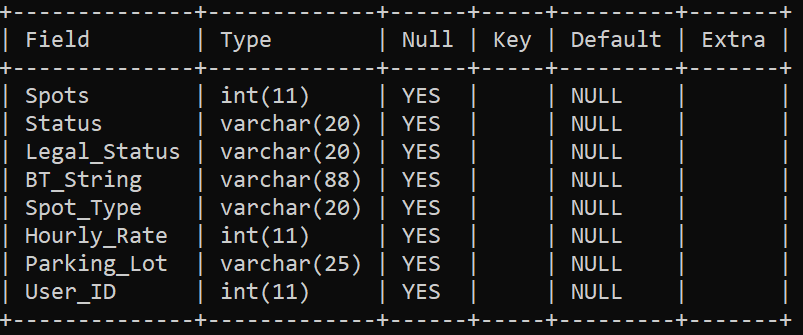
\includegraphics[scale=1]{spacesTable}
\caption{All entries in the Spaces Table}
\label{spaces}
\end{figure}
\subsubsection{\textbf{Users}} The users table keeps track of people who have permits or money on their account along with his/her permit type. Figure \ref{users} describes all fields in the Users table
\begin{figure}[H]
\center
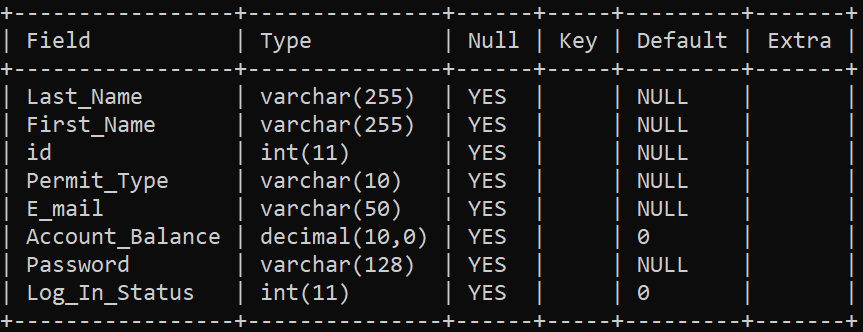
\includegraphics[scale=1]{usersTable}
\caption{All entries in the User Table}
\label{users}
\end{figure}
\subsubsection{\textbf{Transaction History}} The Transaction History table keeps track of every transaction made in a day. It contains User IDs, a time stamp, payment amount, transaction type, parking spot and parking lot. Everytime a user leaves a space or enters a space, the data is logged in this table. A list of fields in this table can be seen in 

\subsubsection{\textbf{Occupation History}} The Occupation history table keeps track of the time of when a spot was occupied and vacant.
%\end{enumerate}
\end{document}